\documentclass[10pt, a4paper, notitlepage, DIV=15]{scrartcl}
\usepackage[ngerman, english]{babel}
\usepackage[utf8]{inputenc}
\usepackage[T1]{fontenc}
\usepackage{csquotes}
\usepackage{xcolor}
\usepackage{amsmath}
\usepackage{amsfonts}
\usepackage{graphicx}
\usepackage{siunitx}
\usepackage{csquotes}
\usepackage{hyperref}


\title{Optical Frequency Doubling}

\author{Max Bock \\ Email \href{mailto:s6mabock@uni-bonn.de}{s6mabock@uni-bonn.de} 
	\and Marvin Hoffmann \\ Email \href{mailto:marvin.hoffmann@uni-bonn.de}{marvin.hoffmann@uni-bonn.de} }




\begin{document}
\maketitle
\tableofcontents
\newpage
\section{Introduction}
In this experiment, the phenomena of frequency doubling will be studied. Frequency doubling is a nonlinear process which can be observed for high intensities of electromagnetic fields. The research field of nonlinear optics is highly active, since it is significant for basic science research as well as for industrial applications. For studying this nonlinear process, the laser beam of a high power diode laser at a wavelength of $987\,$nm in the infrared regime will be frequency doubled with the use of a potassium niobate crystal to visible light at $493,5\,$nm. For this, firstly the properties of the diode laser will be determined. Subsequent, the effect by the power and polarization of the incoming, fundamental wave and by the temperature of the crystal to the frequency doubled light will be observed. Further, the wavelengths ratio of the fundamental and the second harmonic wave will be tried to verify by first the use of a grating and later for more precision also a Michelson interferometer. 
\section{Theory}
\subsection{Diode Laser}
In principle, a diode laser consists of semiconductor materials and operates on transition between electrons in the conduction band recombining with holes in the valence band. The energy, which is released by the recombination, is fractional converted into radiative energy in form of photons. By forward biasing a junction of heavily doped p and n materials, a large density of electrons and holes is produced. The radiation, which is caused by this process, is used for the stimulation of the recombination. \cite{lasers}\newline By changing the applied current, the output power can be tuned. In the range where the gain is equal or higher than the losses such that the gain satisfies the lasing condition, the power increases linearly with the applied current. In figure \ref{fig:threshold}, the output power in dependence of the applied current is presented. Before the threshold current, the output power results from the spontaneous emission, whereupon after the lasing threshold, the stimulated emission causes the lasing output.  
\begin{figure}[h]
	\centering
	\includegraphics[width=0.6\textwidth]{threshold}
	\caption{Laser power with respect to applied current. At the threshold current, lasing action starts.}
	\label{fig:threshold}
\end{figure}
\newline
The output power $P_{out}$ in the linear regime is then given by \cite{laserphysics}
\begin{equation} \label{eq:threshold_current}
	P_{out} = \frac{I-I_{th}}{e}h\nu
\end{equation} 
with the applied current $I$, the threshold current $I_{th}$ when the gain and the losses balanced reciprocal and every injected electron is add to recombination, the energy of a photon $h\nu$ and the charge of an electron $e$. \label{threshold}  
\newline
The quantum efficiency $\eta$ is defined as the ratio between the number of emitted photons $N_{\gamma}$ and the number of electrons which are crossing the diode junction $N_{e}$ to \begin{equation}
	\eta=\frac{N_{\gamma}}{N_e}
\end{equation}
with the number of emitted photons $N_{\gamma}$ and the number of electrons $N_{e}$ given by
\begin{equation}
	N_{\gamma} = \frac{P\cdot t}{h\nu} \quad \textrm{and} \quad N_e=\frac{I\cdot t}{e}
\end{equation}
This yields to the quantum efficiency given by 
\begin{equation} \label{eq:qmefficiency}
	\eta = \frac{e}{h\nu}\cdot \frac{P}{I}
\end{equation} \cite{quantumefficiency}
\newline
\subsection{Generation of Harmonics by Nonlinearities}
In linear optics, the refractive index and the absorption coefficient, which describe the dispersion of light in matter, are independent of the intensity of the incoming field. From this follows two important principles like the superposition principle and the conservation of frequency. These both principles do not count anymore for high intensities. \newline
In a linear medium, the polarisation is described by
\begin{equation} \label{polarisation_linear}
P(\omega)=\epsilon_0 \chi(\omega)E(\omega)
\end{equation}
with the electric field constant $\epsilon_0$, the electric susceptibility $\chi(\omega)$ and the complex electric field $E(\omega)$. This implies that the electrons of the atoms are bounded in a harmonic parabola potential. However, in reality this is only an approximation to the real potential which is presented in figure \ref{fig:potential}.
\begin{figure}[h]
	\centering
	\includegraphics[width=0.6\textwidth]{potential}
	\caption{Comparison of the ideal with the real potential. $U$ describes the potential, $d$ the deflection of the electron. and $E_b$ shows the binding energy of the electron.   \cite{bergmann}}
	\label{fig:potential}
\end{figure}
\newline
For high intensities, the deviations of both potentials are recognizable. In the case of high intensities the polarisation cannot described anymore by equation but is a function of the electric field and therefore consists further of terms with higher orders. By assuming e.g. a cosine electric field, the polarisation is given by
\begin{equation}
P=P^{(0)}+P^{(1)}(\omega)+P^{(2)}(2\omega)
\end{equation}
so the polarisation consist in addition to the fundamental wave $P^{(1)}(\omega)$, further of the direct component $P^{(0)}$ and a component of the second harmonic generation with the doubled frequency $P^{(2)}(2\omega)$. Due to energy conservation it can be calculated that two fundamental waves create  one second harmonic wave, which is illustrated in figure \ref{fig:wavedoubling}.
\begin{figure}[h]
	\centering
	\includegraphics[width=0.6\textwidth]{wavelengthdoubling.png}
	\caption{Illustration of frequency doubling, especially the fact that two fundamental waves (with wavelength $\omega_1$) create one second harmonic wave (with wavelength $\omega_2=2\omega_1$) \cite{boyd} - edited}
	\label{fig:wavedoubling}
\end{figure}
\newline Non-linear behaviour was first researched theoretically in the years 1927 and 1931 but the first experimental evidence of non-linear process was observed since the invention of the laser whereupon frequency doubling was possible in 1961. \newline
In this experiment the non-linear effect  of frequency doubling will be considered. Therefore, the fundamental wave with a high intensity will be irradiate into a crystal. This phenomenon occurs since the electric field forces the electrons to move non-harmonically so the amplitude consists of higher frequency orders. The second harmonic wave with the doubled frequency can appear if the inversion symmetry of the crystal is broken.\cite{bergmann}
\newline
The intensity for the second harmonic wave is given by \cite{meschede}
\begin{equation}\label{eq:ishg}
I_{shg} = \Gamma L^2 I_{fun}^2 \left( \frac{\sin(\Delta k L / 2)}{\Delta k L / 2} \right)^2,
\end{equation}
where $\Gamma$ is a material depending variable, $L$ is the length of the crystal and $I_{fun}$ is the intensity of the fundamental wave. $\Delta k$ is the so called phase mismatching, which will be explained in the next paragraph. So the intensity of the second harmonic wave is proportional to the square of the intensity of the fundamental wave. \newline
As seen in formula \ref{eq:ishg} the intensity of the second harmonic does not just depend on the square of the length of the crystal. This is due to the fact that the refraction index of the crystal depends on the wavelength of the beam, what means that the refraction index of the second harmonic wave $n_{shg}$ is not equal to the refraction index of the fundamental wave $n_{fun}$. That leads to different velocities for the fundamental and the second harmonic wave inside the crystal, so that there will be constructive and destructive interferences. From this follows the phase mismatching \cite{meschede}
\begin{equation}
\Delta k = k_{shg}-2k_{fun} = \frac{2\omega}{c}(n_{shg}-n_{fun}),
\end{equation}
where $c$ is the speed of light, $\omega$ is the frequency of the fundamental beam and the $k$s are the wave numbers of the fundamental and the second harmonic wave. The effective interaction length is called coherence length $l_{coh}$ and is given by\cite{meschede}
\begin{equation}
l_{coh}=\frac{\pi}{\Delta k}.
\end{equation}  
\newline It is obvious that there is a maximum in the second harmonic intensity for a vanishing $\Delta k$, which means for equal refraction index for the fundamental and the second harmonic wave. The most common way to ensure this is by making use of birefringence media, to compensate the difference in wavelength depending refraction index. 
\subsection{Birefringence and Retardation Plates}\label{sec:birefring}
Birefringent materials are optically anisotropic, which means, that their optical properties are not the same in all directions. That leads to polarization depending refraction indexes.\cite{hecht}\newline
The easiest case of optically anisotropic material is an uniaxial crystal with one axis of symmetry, which is often called optical axis. Light rays whose polarization is perpendicular to the optic axis are called ordinary rays whereby rays whose polarization is in the direction of the optical axis are called extraordinary rays. The refraction index of the ordinary and extraordinary rays are given by $n_o$ and $n_e$, whereas in general $n_o \neq n_e$.\newline
Every beam in an uniaxial crystal will be separated into two beams, an ordinary and an extraordinary beam. Because of the different refraction indexes, these two beams have not longer the same velocity, which leads to different propagation direction and a drifting apart, the so called beam walk-off.\newline
A important usage of birefringence materials are retardation plates, which are used to change the polarization of beams. In this case, the optical axis is perpendicular to the propagation direction. An incoming linear polarised beam is separated into an ordinary and an extraordinary beam and their components are given by the projection on the optical axis. These two beams are propagating with two different velocities, due to the fact that the refraction indexes of are not equal. That leads to a deviation in optical path length for the ordinary and extraordinary beam.\cite{meschede} 
\newline If this distinction of the optical path length is half of the wavelength of the incoming beam, the polarisation of the outgoing beam is polarized around the optical axis. Retardation plates, which fulfils this criterion are called half-wave plate or $\lambda/2$-plate. By rotating the alignment of the optical axis of the $\lambda/2$-plates it is possible to rotate the linear polarization of an incoming beam in every direction.\cite{hecht} 
\subsection{Phase Matching}
As described before, the maximum intensity of the second harmonic wave is reached for a vanishing phase mismatching $\Delta k$, which means that $n_{fun}=n_{shg}$ must be fulfilled. For crystal with normal dispersion, the refraction index is higher for smaller wavelengths, so that $n(\omega_{fun})<n(\omega_{shg})$.
\newline One way to reach phase matching is to make use of birefringence crystals for the frequency doubling. As discussed in section \ref{sec:birefring}, birefringence crystals have (in the easiest case) two different refraction indexes, the ordinary and the extraordinary refraction index $n_o$ and $n_e$. That means that the second harmonic wave has to be the extraordinary beam for negative uniaxial crystals ($n_e<n_o$) or the ordinary beam for a positive uniaxial crystal ($n_e>n_o$) to reach phase matching. In these cases phase matching is reached, if the polarization of the fundamental wave is complementary to the second harmonic wave. This type of phase matching is defined as type I phase matching by Midwinter and Warner (1965) \cite{boyd}. It is called type II phase matching if the polarization of the fundamental wave is separated into the ordinary and extraordinary axis. \cite{meschede}

\subsection{Gaussian Beams}
The beam of a laser which is working in ground mode shows a Gaussian intensity distribution. A typical parameter of a gaussian beam is the beam waist $w(0)$ which is defined as the minimal beam radius $w(z)$. \cite{kühlke}\newline
The distribution of a Gaussian beam is shown in figure \ref{fig:gauss}.
\begin{figure}[h]
	\centering
	\includegraphics[width=0.6\textwidth]{gaussian_beam}
	\caption{Profile of a Gaussian beam with characteristic properties. \cite{wiki_gauss}}
	\label{fig:gauss}
\end{figure}
\newline
\\
- shape of laser beam has gaussian shape 
- figure of gaussian beam
- diameter of gaussian beam $w(z)=w0\sqrt{1-\frac{z^2}{z0^2}}$ $w0$= beam waist $z_0$ Rayleigh length 
- confocal parameter $b=2z0$
\subsection{Determination of Wavelengths with Gratings}
-Gittergleichung (eher in analysis)
\subsection{Michelson Interferometer}
-description in set-up
\section{Experimental Set-Up and Measurements}
\subsection{Diode Laser and Power Measurement}
Firstly, the properties of the diode laser will be measured. The diode laser is a commercial, external cavity diode system will a grating in Littrow configuration. The laser has a high intensity of up to $180\,$mW at a wavelength of $987\,$nm, since high intensities are necessary to study nonlinear processes. For reasons of safety, a shutter is placed directly behind the laser system to shield the beam when the shutter is closed. With a prism pair the elliptic beam is converted into a more round shape.
\subsubsection{Laser Output Power vs. Injection Current}
First of all, the laser output power is measured in dependence of the injection current. The experimental set-up is depicted in figure \ref{fig:power_fun}.
\begin{figure}[h]
	\centering
	\includegraphics[width=0.6\textwidth]{power_fun}
	\caption{Set-Up for measuring the Output Power. \cite{description}}
	\label{fig:power_fun}
\end{figure}
\newline
Since the powermeter becomes nonlinear for powers above $20\,$mW, an attenuator is used to reduce the power. For determining the attenuation factor, the applied current is at first increased up to a measured power shortly before the nonlinear region is reached without attenuator and then is repeated again for the same values of the applied current but with the use of the attenuator. \newline
Afterwards, the applied current is increased further up to $280\,$mA while the output power is measured with the help of the attenuator.
\subsubsection{Calibration of the variable Attenuator}
The laser is not stabilize while changing the applied current to the diode, so mode hops can occur. For prevent these mode hops, the variation of the output power will be performed without changing the injection current, but by the use of a $\lambda/2\,$-plate and a polarizer. The set-up is presented in figure \ref{fig:cal_atten}.
\begin{figure}[h]
	\centering
	\includegraphics[width=0.8\textwidth]{cal_atten}
	\caption{Set-Up for Calibration of the variable Attenuator. \cite{description}}
	\label{fig:cal_atten}
\end{figure}
\newline
The $\lambda/2\,$-plate is mounted in a rotatable holder and so by changing the rotation angle of the plate, the polarization angle of the linear polarized light is rotated. Since the polarizer transmits only one polarization component, the power of the fundamental wave can be changed by this method. \newline
While changing the rotation angle of the $\lambda/2\,$-plate in steps of $2.5^\circ$ the power of the fundamental wave is measured.
\subsection{Focussing the Laser Beam into the Crystal and Optimizing the Harmonic Power}
Afterwards, the frequency doubling process will be studied. Therefore, the potassium niobate crystal is placed inside the laser beam.
\subsubsection{Optimization of Second Harmonic Power}
The collimated beam is focussed in the crystal by the use of a plano-convex lens with a focal length of $f=60\,$mm. For optimizing the second harmonic wave, the temperature of the crystal is increased by a temperature-stabilizing device to $36^{\circ}\,$C which will later be seen is the optimal temperature for phase matching of the fundamental and second harmonic wave. The second harmonic wave is first roughly optimized by changing the distance between the focussing lens and the crystal to get the focal point in the middle of the crystal. Subsequently, an achromatic lens with a focal length of $f=60\,$mm is used to collimate the frequency doubled light and a $3\,$mm BG40 glass filter is used to filter out the infrared light. Then for fine optimization, the power of the second harmonic wave is measured with the power meter which is protected with a straylight shielding tube and the crystal while the position of the crystal is optimized. The experimental set-up for the measurement of the second harmonic power is depicted in figure \ref{fig:power_sec_harm}.
\begin{figure}[h]
	\centering
	\includegraphics[width=1\textwidth]{power_sec_harm}
	\caption{Set-Up for measuring Second Harmonic Power. \cite{description}}
	\label{fig:power_sec_harm}
\end{figure}
\newline
\subsection{Properties of Second-Harmonic Generation}
After the phenomena of frequency doubling is optimally observable, the effects by the temperature of the crystal as well as the effects by the power and polarization of the fundamental wave to the harmonic wave are studied. The set-up for these measurements is shown in figure \ref{fig:power_sec_harm}.
\subsubsection{Harmonic Power vs. Crystal Temperature}
Firstly, the temperature of the crystal is reduced to $27^{\circ}\,$C and then slowly increased in steps of $0.2^{\circ}\,$C up to $40^{\circ}\,$C while the power of the second harmonic wave is measured.
\subsubsection{Harmonic Power vs. Fundamental Power}
The temperature of the crystal will be setted to the optimum value which was in this experiment at $36^{\circ}\,$C. The power of the second harmonic wave will be measured while rotating the angle of the $\lambda/2\,$-plate in steps of $2.5^\circ$. 
\subsubsection{Harmonic Power vs. Polarization of Fundamental Wave}
In the end, the polarizer will be removed. Now, by changing the rotation angle of the $\lambda/2\,$-plate not the power but the angle of polarization of the fundamental wave will be changed. While rotating the angle of the $\lambda/2\,$-plate in steps of $2.5^\circ$ the power of the second harmonic wave will be measured.
\subsection{Comparison of the Wavelengths of Fundamental and Harmonic Waves}
\subsubsection{Diffraction grating}
For a first rough comparison of the fundamental and second harmonic wave, a blazed diffraction grating with $600\,$lines/mm is used. The set-up for this part of the experiment is shown in figure \ref{fig:grating}.
\begin{figure}[h]
	\centering
	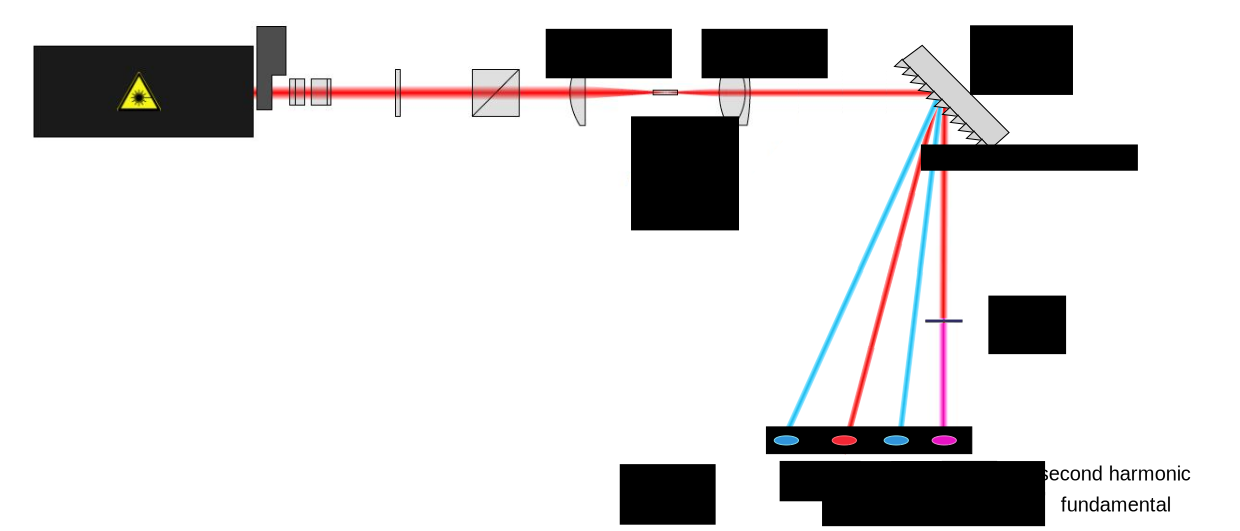
\includegraphics[width=1\textwidth]{grating}
	\caption{Set-Up for Comparison of the Wavelengths of Fundamental and Harmonic Waves with blazed Diffraction Grating. \cite{description} - edited}
	\label{fig:grating}
\end{figure}
\newline
By the grating inside the optical path, different diffraction orders of the fundamental and the second harmonic wave appear and are observable at the wall. For a higher resolution, the achromatic lens with a focal length of $f=60\,$mm is replaced by the achromatic lens with the largest focal length of $f=125\,$mm to illuminate the most lines on the grating and is aligned properly to get the smallest beam diameter at the screen. By comparing the diffraction angles between the $n$-th order of the fundamental and the $2n$-th order of the second harmonic wave, the ratio between the both wavelengths can be determined. For better observation of the second harmonic wave, the $3\,$mm BG filter is used to reduce the intensity of the fundamental wave. 
\subsection{Interferometric Comparison using Michelson Interferometer}
For a more precise comparison of the both wavelengths, a Michelson interferometer is built up and properly aligned. A sketch of the set-up is shown in \ref{fig:michelson}.
\begin{figure}[h]
	\centering
	\includegraphics[width=1.05\textwidth]{michelson}
	\caption{Set-Up for the Two-Colour Michelson Interferometer. \cite{description}}
	\label{fig:michelson}
\end{figure}
\newline
For the interferometer, two partially transmitting beam splitters and two end mirrors are used. One of the end mirrors is fixed while the other one is mounted on a movable slide. By this, it is possible to change the optical path length of one arm of the interferometer. The reflection of the fundamental beam back into the laser is prevented by a $1\,$mm  BG filter which is placed after the collimating lens. Since the interferometer works best with a collimated beam with a small beam diameter, the achromatic lens with the largest focal length of $f=125\,$mm is replaced by the achromatic lens with the smallest focal length of $f=30\,$mm. The beam splitter splits the incoming beam such that a part of the beam goes to the fixed end mirror and the other part of the beam is travelling to the movable end mirror. The back reflecting parts overlap at the output of the interferometer which is observed at the the white wall first which acts like a screen. The mirrors are aligned such that an interference pattern is observable which becomes brighter and darker for a really short change in the path difference of a few hundred nanometres by pressing on the optical table. After perfect alignment, the $3\,$mm thick BG filter is placed at the output of the interferometer at $45^\circ$ to the beam wo separate the fundamental and the second harmonic waves. The transmitted second harmonic beam and the reflected fundamental beam are measured with two photodiodes which are connected to an oscilloscope. The oscilloscope presents the both signals in x-y mode to observe Lissajous figures. By changing the position of the movable end mirror different Lissajous figures are observable.
\section{Analysis}
\subsection{Diode Laser and Power Measurement}
\subsubsection{Laser Output Power vs. Injection Current} \label{threshold_current}
For the analysis of the power of the fundamental wave, the attenuation factor has to be determined. Therefore, eight times the output power of the laser is measured with ($P_{att}$) and without attenuator ($P$) for the same values of the applied current $I$. The systematic errors of the power measurement are estimated to $\Delta P_{(att)} = 0.03 \cdot P\,$ since the values fluctuate in dependence of the measured power. This error is caused by the instability of the laser, so intensity and wavelengths fluctuate due to mode hops. Further, the powermeter and the sensor cause fluctuations in the measurement. The measured output power is corrected by the background measurement $P_{back}$. For the case of the measurement without attenuator, a background radiation power of $P_{back}=9\,$mW is measured and for the measurement with attenuator, a background radiation power of $P_{back}^{att}=6\,$nW is measured. The errors of the background measurement are also estimated to $\Delta P_{back}^{(att)}=3\%$ for the same reason mentioned above. The error of the corrected output power is calculated by Gaussian error propagation with 
\begin{equation}
	\Delta P_{corr}^{(att)}= \sqrt{\left(\Delta P^{(att)} \right) ^2 + \left(\Delta P_{back}^{(att)} \right) ^2}
\end{equation}
In the following, all errors are calculated by Gaussian error propagation if not explicitly mentioned differently. The attenuation factor $A$ is calculated for each of the eight measurements with
\begin{equation}
	A=\frac{P_{corr}}{P_{corr}^{att}}
\end{equation}
and then averaged to
\begin{equation}
	A_{ave}=\frac{1}{8}\cdot\sum_{i=1}^{8}A_i
\end{equation}
The error of the averaged attenuation factor is estimated by the standard deviation. Therefore, an average attenuation factor of
\begin{equation}
	A_{ave}=1661\pm 110
\end{equation}
is estimated. All discussed values are presented in the appendix in section \ref{values_fun}. \newline
Further, the power of the fundamental wave is measured by the use of the attenuator $P_{att}$ and then corrected by background with the same procedure mentioned above to $P_{corr}^{att}$. For determining the threshold current and the quantum efficiency, the real output powers of the laser have to be calculated. Therefore, the measured power with the attenuator $P_{corr}^{att}$ is corrected by the average attenuation factor $A_{ave}$ with
\begin{equation}
	P=P_{corr}^{att}\cdot A_{ave}
\end{equation}
The real power $P$ is plotted in dependence of the applied current $I$ whereupon the systematic error of the current is estimated to $\Delta I = 0.5\,$mA since it was possible to change the current in steps of $1\,$mA. The plot of this measurement is shown in figure \ref{fig:output_pow_current}.
\begin{figure}[h]
	\centering
	\includegraphics[width=1\textwidth]{Gnuplot/fun_current}
	\caption{Measurement of the output power $P$ in dependence of the applied current $I$.}
	\label{fig:output_pow_current}
\end{figure}
\newline
By fitting a linear function $f(x)=m\cdot x +b$ to the data in the range where the power increases linearly, one can determine the threshold current and the quantum efficiency. The threshold current $I_{th}$ with respect to equation \ref{eq:threshold_current} is given by
\begin{equation}
I_{th}= - \frac{b}{m}
\end{equation}
with received fit parameters $b=\left( -30.8 \pm 0.6 \right)\,$ mW and the differential slope efficiency $m=\left( 0.564 \pm 0.003  \right)\, $ W/A and a reduced chisquare of $\chi^2=4.60$. Thereby, it follows that the threshold current for this diode laser is given by
\begin{equation}
I_{th}=\left( 55\pm 1\right)\,\text{mA}
\end{equation}
The quantum efficiency is determined by equation \ref{eq:qmefficiency} and the assumption that 
\begin{equation}
\frac{P}{I} \approx \frac{\partial P}{\partial I} = m
\end{equation}
which is fulfilled in the linear range.
This yields to a differential quantum efficiency
\begin{equation}
\eta = \frac{e}{h \nu} \cdot m
\end{equation}
with the frequency $\nu=c/\lambda$. With $\lambda=987\,$nm follows $\nu=3.04\cdot10^{14}$.
From this, the quantum efficiency for this diode laser is calculated to
\begin{equation}
\eta = 0.449 \pm 0.002
\end{equation}
\subsubsection{Calibration of the variable Attenuator}
As discussed above, the power of the fundamental wave is from now on not changed by changing the applied current since mode hops occur but by using the $\lambda/2\,$-plate and the polariser. Firstly, the power of the fundamental wave $P_{fun}$ is measured in dependence of the rotational angle $\theta$ of the $\lambda/2\,$-plate. The power of the fundamental wave is corrected with the background measurement and by taking into account the average attenuation factor $A_{ave}$ as already mentioned in section \ref{threshold_current}. In addition, the same systematic errors for the measurement with the powermeter are estimated as before to $\Delta P = 0.03\cdot P$. The systematic error of the rotation angle is estimated to $\Delta \theta=1.25^\circ$ due to metering since the centre between two scale divisions was at $2.5^\circ$ at the rotation plate of the $\lambda/2\,$-plate so in each direction $\pm 1.25^\circ$. The transmitted intensity of a linear polarised wave after a polariser is described by the law of Malus which is given by \cite{zinth}
\begin{equation}
	I(\theta)=I_0\cdot \cos^2(\theta)
\end{equation}
with the initial intensity $I_0$ and $\theta$ the angle between the initial polarization direction of the light and the axis of the polariser. Due to that, a cosine-squared behaviour of the measured power $P_{fun}$ after the polariser for different rotation angles $\theta$ of the $\lambda/2$-plate is expected. A plot of this measurement is shown in figure \ref{fig:output_pow_angle}. Therefore, the angles in degrees are converted to radians.
\begin{figure}[h]
	\centering
	\includegraphics[width=1\textwidth]{Gnuplot/fun_angle}
	\caption{Measurement of the fun $P$ in dependence of the rotation angle $\theta$ of the $\lambda/2$-plate.}
	\label{fig:output_pow_angle}
\end{figure}
\newline
By fitting a cosine-squared function to the data with $f(x)=a\cdot \cos^2(b\cdot x+c)+d$, the fit parameters were determined to $a=(203 \pm 2) \,$mW, $b= (1.997 \pm 0.003)\,$, $c = (-0.856 \pm 0.006)\,$ and $d= (0.73 \pm 0.05)\,$mW with a reduced chisquare of $\chi^2=1.54$. The ratio between maxima and minima is described by $a$ and $d$, whereupon the maxima can be calculated by $P^{max}_{fun}=a+d$ and the minima by $P^{min}_{fun}=d$. The extinction ratio $R$ defined as maximum and minimum of the transmitted power is then given by 
\begin{equation}
	R=\frac{a+d}{d}=279\pm 19
\end{equation}
The parameter $b$ is the compression factor and $c$ the relative phase.
\subsection{Focussing the Laser Beam into the Crystal and Optimizing the Harmonic Power}
\subsubsection{Optimization of Second Harmonic Power}
\subsection{Properties of Second-Harmonic Generation}
\subsubsection{Harmonic Power vs. Crystal Temperature}
\subsubsection{Harmonic Power vs. Fundamental Power}
\subsubsection{Harmonic Power vs. Polarization of Fundamental Wave}
\subsection{Comparison of the Wavelengths of Fundamental and Harmonic Waves}
\subsubsection{Diffraction grating} 
\subsection{Interferometric Comparison using Michelson Interferometer}
\section{Conclusion}
\section{Appendix}
\subsection{Diode Laser and Power Measurement}
\subsubsection{Laser Output Power vs. Injection Current} \label{values_fun}  
(\textcolor{red}{here table of values in appendix})
\begin{thebibliography}{}
\bibitem{lasers}
	Peter W. Milonni (Los Alamos National Laboratory) and Joseph H. Eberly (University of Rochester), \textit{Lasers} (Wiley-Interscience, 1988)
\bibitem{laserphysics}
	Simon Hooker and Colin Webb, Department of Physics, University of Oxford, \textit{Laser Physics}, (Oxford University Press, 2011)
\bibitem{quantumefficiency}
Massachusetts Institute of Technology (MIT), Electrical Engineering and Computer Science, Compound Semiconductor Devices, 2003 \url{https://ocw.mit.edu/courses/electrical-engineering-and-computer-science/6-772-compound-semiconductor-devices-spring-2003/lecture-notes/lecture20.pdf}
\bibitem{bergmann}
	Bergmann and Schäfer, \textit{Lehrbuch der Experimentalphysik, Band 3, Optik und Wellenmechanik}, de Gruyter Verlag, 10th. edition (2004)
\bibitem{boyd}
	R. W. Boyd, \textit{Nonlinear Optics}, Academic Press Boston (1992)
\bibitem{meschede}
D. Meschede, \textit{Optik, Licht und Laser}, Vieweg+Teubner Verlag, 3.rd edition (2008)
\bibitem{hecht}
	E. Hecht, \textit{Optics}, Addison Wesley, 4.th edition (2002)
\bibitem{kühlke}
	D. Kühlke, \textit{Optik - Grundlagen und Anwendungen}, Verlag Harri Deutsch, 3.rd improved edition (2011)
\bibitem{wiki-gauss}
	\url{https://en.wikipedia.org/wiki/Gaussian_beam#/media/File:GaussianBeamWaist.svg}
\bibitem{description}
	Experimental Description, \textit{A245: Optical Frequency Doubling}, University of Bonn, August 2015
\bibitem{zinth}
	W. Zinth and U. Zinth, \textit{Optik} \textit{Lichtstrahlen-Wellen-Photonen}, Oldenbourg Verlag München, 4th. improved edition (2013)
	

\end{thebibliography}
 
\end{document}